\documentclass[12pt,letterpaper]{article}
\usepackage[utf8]{inputenc}
\usepackage[T1]{fontenc}
\usepackage[activeacute,spanish]{babel}
\usepackage[left=18mm,right=18mm,top=21mm,bottom=21mm,letterpaper]{geometry}%
\usepackage{helvet}
\usepackage{amsmath,amsfonts,amssymb,commath}
\usepackage{graphicx}
\usepackage{color}
\usepackage{xcolor}
\usepackage{verbatim}
\usepackage{tabls}
\usepackage[space]{grffile}
\usepackage{url}
\usepackage{listings}
\usepackage{circuitikz}
\usepackage{siunitx}

\usepackage{matlab-prettifier}

\usepackage{textcomp}
\usepackage{booktabs}
\usepackage[colorlinks=true,urlcolor=blue,linkcolor=black,citecolor=black]{hyperref} 
\usepackage{pdfpages}   %incluir paginas de pdf externo, para los anexos
\usepackage{caption}
\usepackage{subcaption}  
\usepackage{rotating}
\usepackage[section]{placeins}
\usepackage{tikz}

\begin{document}

\title{Laboratorio 1 MATLAB}
\author{Daniel García Vaglio (B42781), Esteban Zamora (B47769), Ariel Fallas (B42481)}
\maketitle

\section{Ejercico 1}


Para esta parte se generó un script el cual ejecuta los comandos en el orden solicitado, se pide graficar ciertas funciones ya dadas, todas dentro de una misma gráfica, esto es muy sencillo ya que lo único que se hace es definir las funciones y1 , y2 , .... , y12 . Los cuales dependen de las entradas definidas x1 , x2 , ...., x12 respectivamente. Y finalmente mediante la función ''plot()'' podemos generar la gráfica de ''y'' contra ''x'' .El único incoveniente que se tenía fue con la función y10 ya que estabagraficando únicamente un punto, ya que únicamente estaba recibiendo un valor, de esta forma matlab no detectaba que era un vector y por ello a la hora de graficarlo se denotó.  esto en código se ve así.
Para lograr el color solicitado únicamente se debía especificar ''r (red)'' o ''y de (yellow)'' dentro de la función de plot como venía en la documentación de la función.

\subsubsection{Código de ejercicio 1}


Script principal:
\lstinputlisting[style=Matlab-editor, basicstyle=\mlttfamily]{Ejercicio1.m}



\section{Ejercicio 2}
En esta sección se comenzó a explorar un poco más las funciones de matrices, ya que todos los objetos son formados a partir de matrices. Para esto se buscó la documentacion de algunas funciones necesarias como lo fue ''randi()'' el cual es un generador de números aleatorios enteros donde puedo especificar el tamaño de la matriz donde quiero que los genere y tambien el rango de valores entre los cuales deseo que vairíen los números generados.\\
A continuación se calcularon los valores y vectores propios para la matriz A. Para obtener los valores propios aplicamos la función ''eig()'', esto genera una columna de valores propios. Sin embargo si lo colocamos en una matriz como para el caso de Vecprop, obtenemos un vector propio por cada columna de la matriz.\\
Al igual que en el primer punto la matriz B se generó apartir de la función ''randi()''.


\section{Ejercicio 3}

Para la primera parte de este ejercicio se pide implementar una función  que encuentre el valor de de la derivada de los estados si se tiene un tiempo y los estados en ese tiempo dado. Esto se implementa en la función derivadasEstados, esta acepta el tiempo y el vector de estados en ese instante, y con esta información calcula la derivada de los estados en ese instante utilizando las ecuaciones (\ref{eq:diferencial1}) y (\ref{eq:diferencial2}). 

\begin{equation}
\frac{dP(t)}{dt}=0,01kP(t)-0,00001aP(t)D(t)
\label{eq:diferencial1}
\end{equation}

\begin{equation}
\frac{dD(t)}{dt}=0,01mD(t)-0,0001bD(t)P(t)
\label{eq:diferencial2}
\end{equation}

En el caso particular de este grupo el número de carné seleccionado es B47769, de manera que $m=9$ $k=7$ $a=4$ y $b=6$. Para resolver la ecuación diferencial se utiliza el código presentado en la subsección de código. Lo que se hace es primero asignar las constantes, luego se itera sobre el tiempo y en cada instante se aplica lo descrito por el método de Runge-Kutta. Al final del ciclo, se tiene una matriz z con los valores que toma cada estado en cada instante descrito por el vector t. 

Se grafica el resultado (ver figura \ref{fig:ejercicio_3_caso_1}), y se obtiene la información de la tabla \ref{table:ejercicio31}. Luego se cambian las condiciones iniciales y se vuelve a simular el sistema (ver figura \ref{fig:ejercicio_3_caso_2}), y se obtiene la información de la tabla \ref{table:ejercicio32}.


\begin{table}
\caption{Datos primer caso de valores iniciales}
\label{table:ejercicio31}
\centering
\begin{tabular}{| l | c |}
  \hline
 \multicolumn{2}{|c|}{Depredadores} \\
 \hline
 Valor mínimo &81.05 \\
 Valor máximo &8150\\
 Primer máximo&39.6\\
 Primer mínimo&110.9\\
 Periodo      &105.5\\
 \hline
 \multicolumn{2}{|c|}{Presas} \\
 \hline
 Valor mínimo &11.46\\
 Valor máximo &606.8\\
 Primer máximo&29.93\\
 Primer mínimo&61.7\\
 Periodo      &105.47\\
 \hline
\end{tabular}
\end{table}


\begin{table}
\caption{Datos segundo caso de valores iniciales}
\label{table:ejercicio32}
\centering
\begin{tabular}{| l| c| }
\hline
  \multicolumn{2}{|c|}{Depredadores} \\
\hline
  Depredadores & \\
  Valor mínimo &19.02\\
  Valor máximo &1.118e+04\\
  Primer máximo&69.7\\
  Primer mínimo&157.5\\
  Periodo      &123.3\\
\hline
  \multicolumn{2}{|c|}{Presas} \\
\hline
  Valor mínimo &3.623\\
  Valor máximo &816.2\\
  Primer máximo&60.87\\
  Primer mínimo&93.1\\
  Periodo      &124.03\\
\hline 
\end{tabular}
\end{table}

\begin{figure}
	\centering
	\begin{subfigure}[b]{0.36\textwidth}
		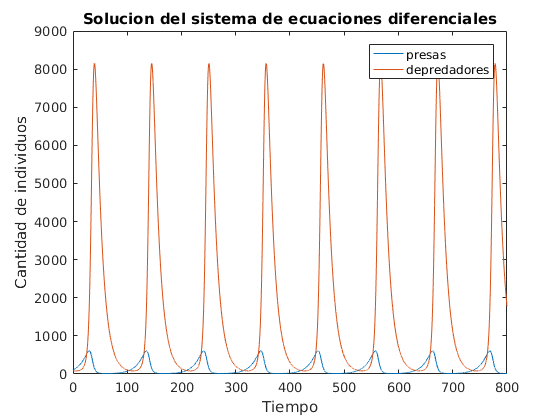
\includegraphics[width=\textwidth]{pictures/ejercicio_3_caso_1}
		\caption{Resultado para primer caso de entradas}
		\label{fig:ejercicio_3_caso_1}
	\end{subfigure}
	\begin{subfigure}[b]{0.36\textwidth}
		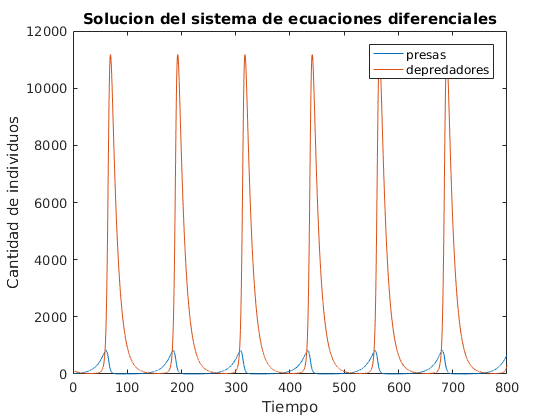
\includegraphics[width=\textwidth]{pictures/ejercicio_3_caso_2}
		\caption{Resultado para segundo caso de entradas}
		\label{fig:ejercicio_3_caso_2}
	\end{subfigure}
        \vfill
        \begin{subfigure}[b]{0.36\textwidth}
		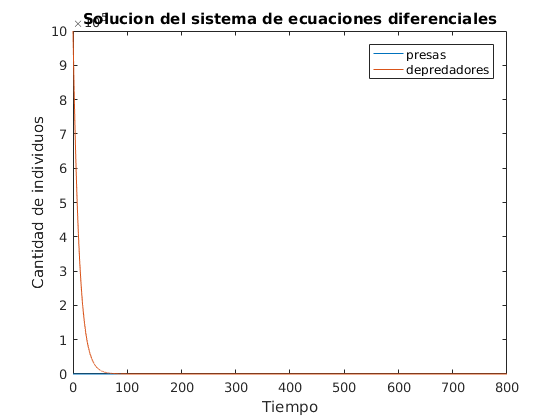
\includegraphics[width=\textwidth]{pictures/ejercicio_3_extincion}
		\caption{Resultado para extinción}
		\label{fig:ejercicio_3_extincion}
	\end{subfigure}
	\caption{Gráficas Ejercicio 3}
	\label{fig:graf_ejercicio_3}
\end{figure}


Note que la solución para los primeros valores iniciales propuestos las funciones tienen una oscilación menor; es decir, las poblaciones se mantienen más estables. Esta condición de estabilidad representa una mejor convivencia de las especies. Además en el segundo caso se tienen incrementos muy elevados de depredadores lo que indica una distribución no equitativa de las poblaciones. En conclusión el primer caso representa una mejor convivencia equitativa entre las especies.

En general, la población de presas tiende a ser menor. También se puede notar que conforme desciende la cantidad inicial de presas mayor amplitud tiene el comportamiento de las poblaciones. Entonces se toma un caso extremo. Con 1000000 depredadores iniciales y 1 presa inicial. Cuando se simula el sistema (ver figura \ref{fig:ejercicio_3_extincion}), es evidente el descenso de ambas poblaciones. En particular se debe notar que la población de presas desciende a menos de 0,5. Como la cantidad de presas es entera, la condición descrita se refiere a 0 presas, lo que implica la extinción. 

\subsection{Código del ejercicio 3}
Script principal:
\lstinputlisting[style=Matlab-editor, basicstyle=\mlttfamily]{Ejercicio3.m}
Función derivadaEstados
\lstinputlisting[style=Matlab-editor, basicstyle=\mlttfamily]{derivadasEstados.m}




\section{Ejercicio 4}



En la figura \ref{fig:diag_bloques}, se muestra el diagrama de bloques que representa 
el modelo en variables de estado propuesto sobre un reactor químico. Tal como se puede 
observar en dicho diagrama, las salidas de los estados $C_a$, $C_b$, $C_x$, $C_y$ y $C_z$ se
encuentran indicadas en las salidas de los bloques integradores. 


\begin{figure}[ht!]
	\centering
	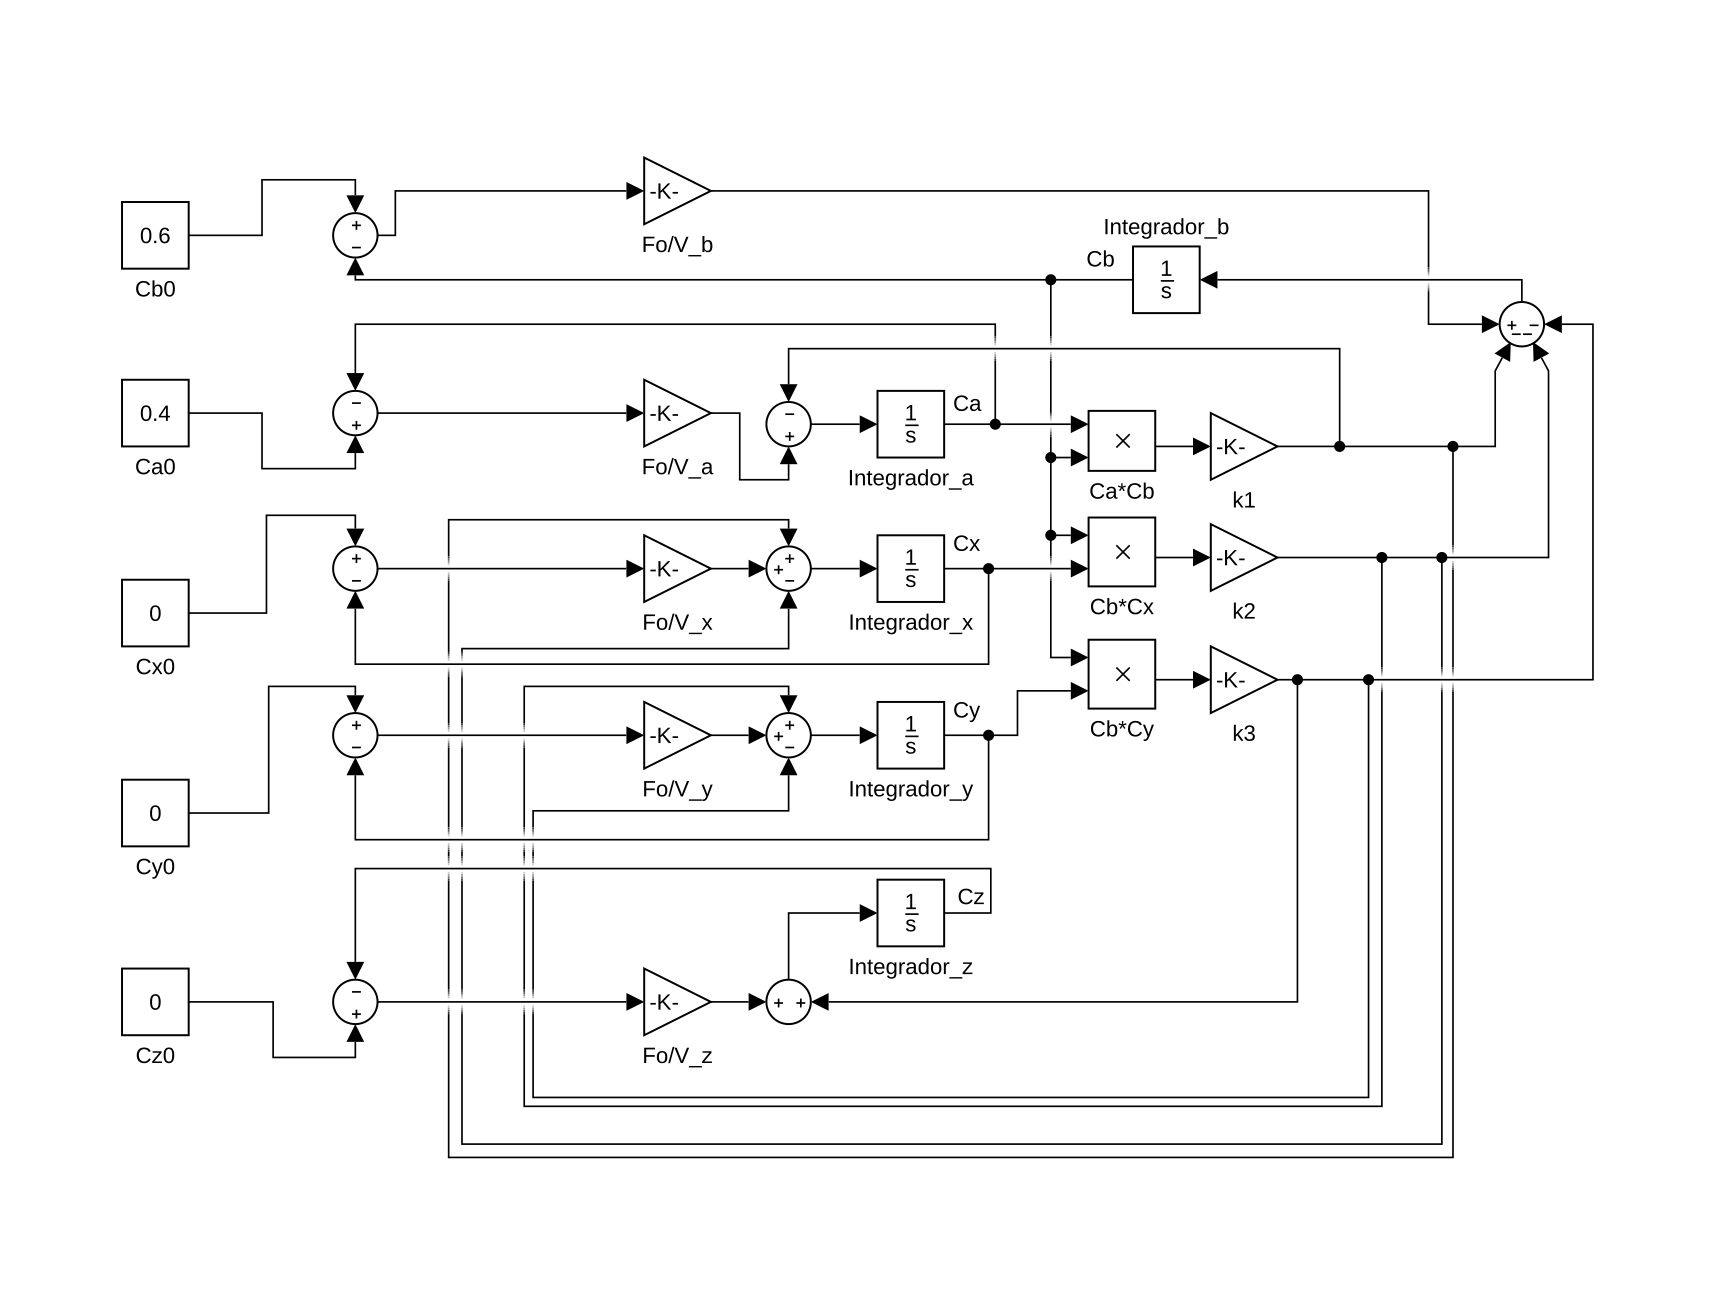
\includegraphics[width=1\textwidth]{pictures/Ejercicio4/diagrama_bloques_2}
	\caption{Diagrama de bloques del MVE del reactor químico}
	\label{fig:diag_bloques}
\end{figure} 



Para generar este diagrama, se partió de las ecuaciones que modelan este sistema. A partir
de esto se observa que para obtener las variables de estado, es necesario integrar una vez cada 
una de estas ecuaciones diferenciales de primer orden, por lo que se colocaron en Simulink los
bloques integradores correspondientes a cada variable.

Luego, se observó que la entrada de cada uno de estos integradores correspondía a la suma y resta de varios 
términos. Para cada ecuación, uno de estos términos dependía de la entrada constante del 
sistema $C_{a0}$, $C_{b0}$, $C_{x0}$, $C_{y0}$ o $C_{z0}$, y de la propia variable de estado, de las
cuales se obtenía su diferencia y esta se multiplicaba por una ganancia $\frac{F_0}{V}$. 
De esta manera, se utilizó el bloque de entrada constante, el bloque de ganancia, un punto de resta
y la retroalimentación de la salida del integrador para generar este término de cada ecuación.


También, de las ecuaciones diferenciales se puede observar que los otros términos en cada ecuación
dependen de una combinación lineal de ciertos productos de los estados en pares, los cuales son
$C_{a}C_{b}$, $C_{b}C_{x}$ y $C_{b}C_{y}$. De esta forma, se utilizó el bloque de multiplicación de
señales para generar estos términos, los cuales se multiplicaron por las ganancias $k_1$, $k_2$ y
$k_3$ respectivamente. 

Finalmente, para completar el diagrama se retroalimentaron los términos descritos previamente a 
los puntos de suma y resta que se encuentran en la entrada de cada uno de los integradores, 
según los términos observados en las ecuaciones del modelo.



Para observar la respuesta de cada una de las variables de estado, se utilizaron los bloques de
\textit{Scope}, de los cuales se obtuvieron las gráficas correspondientes a dichas variables, las
cuales se muestran en la figura \ref{fig:result_mve_reactor}.

\begin{figure}
  \centering
  \begin{subfigure}[b]{0.45\textwidth}
	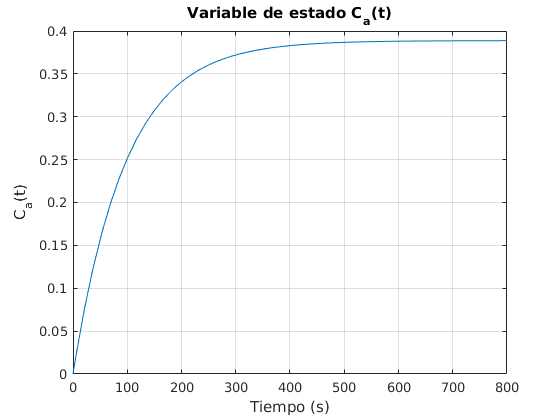
\includegraphics[width=\textwidth]{pictures/Ejercicio4/var_estado_Ca}
	\caption{Gráfica: Variable de estado $C_a$}
	\label{fig:var_estado_Ca}
  \end{subfigure} 

  \begin{subfigure}[b]{0.45\textwidth}
    	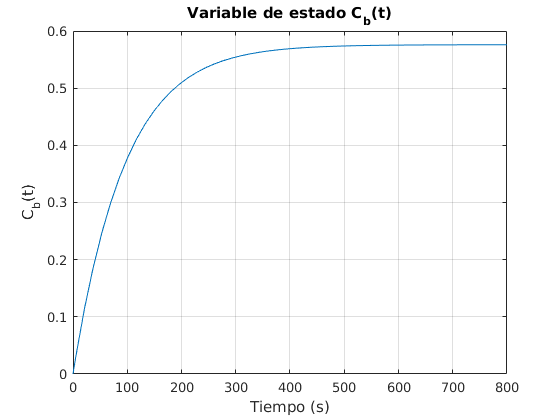
\includegraphics[width=\textwidth]{pictures/Ejercicio4/var_estado_Cb}
	\caption{Gráfica: Variable de estado $C_b$}
	\label{fig:var_estado_Cb}
  \end{subfigure}
  \begin{subfigure}[b]{0.45\textwidth}
	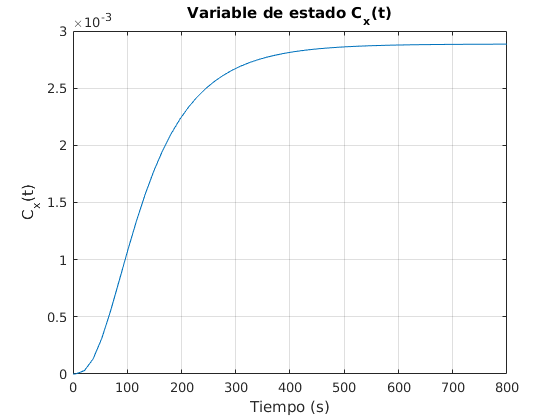
\includegraphics[width=\textwidth]{pictures/Ejercicio4/var_estado_Cx}
	\caption{Gráfica: Variable de estado $C_x$}
	\label{fig:var_estado_Cx}
  \end{subfigure}
  \vfill
  \begin{subfigure}[b]{0.45\textwidth}
	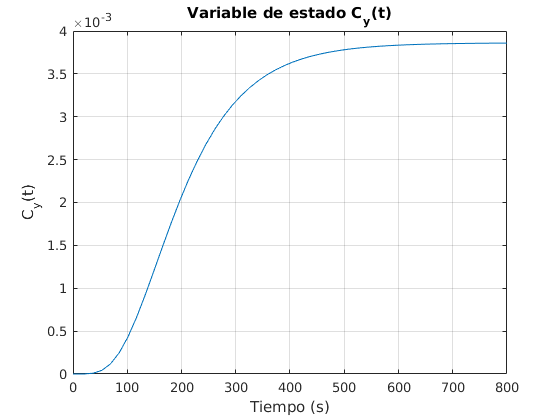
\includegraphics[width=\textwidth]{pictures/Ejercicio4/var_estado_Cy}
	\caption{Gráfica: Variable de estado $C_y$}
	\label{fig:var_estado_Cy}
  \end{subfigure}
  \begin{subfigure}[b]{0.45\textwidth}
	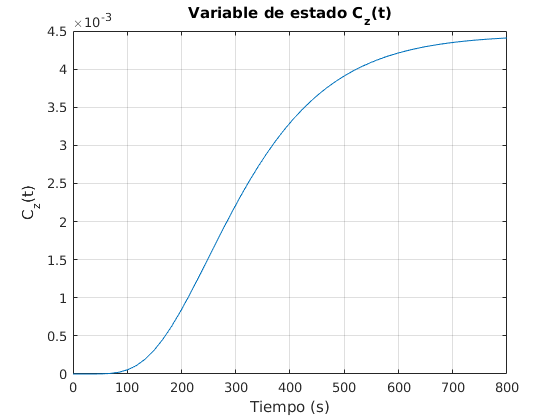
\includegraphics[width=\textwidth]{pictures/Ejercicio4/var_estado_Cz}
	\caption{Gráfica: Variable de estado $C_z$}
	\label{fig:var_estado_Cz}
  \end{subfigure}

  \caption{Resultados de la simulación de las variables de estado del reactor químico}
  \label{fig:result_mve_reactor}
\end{figure}

Para generar estas gráficas, se importaron los datos de estos resultados desde Simulink a MATLAB,
donde luego se generaron las figuras correspondientes según el siguiente código, en donde se muestra
como ejemplo la generación de la gráfica del estado $C_a$:


\begin{lstlisting}[style=Matlab-editor, basicstyle=\mlttfamily]
  figure
  plot(tout, Ca(:,2))
  grid on
  title('Variable de estado C_a(t)')
  xlabel('Tiempo (s)')
  ylabel('C_a(t)')
\end{lstlisting}

Es importante mencionar, que el sistema modelado de este reactor químico no corresponde a un sistema
lineal, por lo que no es posible modelarlo según las ecuaciones matriciales que se utilizan
normalmente al construir los modelos en variables de estado. De esta forma, se muestra que la
utilización de los diagramas de bloques de Simulink constituye una buena herramienta para simular la
respuesta de estos sistemas no lineales.

\section{Ejercicio 5}

Para este ejercicio se procedió a definir en MATLAB las matrices correspondientes a A, B, C y D,
según el modelo propuesto en la guía de esta práctica. El siguiente código muestra la definición de
estas matrices:

\begin{lstlisting}[style=Matlab-editor, basicstyle=\mlttfamily]
  % Matrices del MVE del sistema
  A = [-4, -1, 0, 3, -2, 0;  -1, -2, 1, 0, 4, 3;     3, 0, -3, 2, -1, 2; 
      -3, 0, -4, -2, 1, -1;   1, -5, 0, -2, -1, -2; -1, -3, -3, 0, 1, -1];
  B = [-2; -1; -3; 0; 8; 3];
  C = [-1, -1, 1, -1, 0, 1];
  D = -1;
\end{lstlisting}


Luego, se definió la variable G mediante la función \texttt{ss}, la cual genera un objeto que
contiene la representación en el espacio de estados del sistema, a partir de las matrices A, B, C y
D. También, mediante la variable G se obtuvieron los polos y ceros correspondientes al
sistema. En el siguiente código se muestra la generación del mapa de polos y ceros de la 
figura \ref{fig:diag_polos_ceros}.

\begin{lstlisting}[style=Matlab-editor, basicstyle=\mlttfamily]
  % Representacion en el espacio de estados del sistema
  G = ss(A,B,C,D);
  % Polos del sistema
  P = pole(G);
  % Ceros del sistema
  Z = zero(G);
  % Diagrama de polos y ceros
  h = pzplot(G); 

\end{lstlisting}

En este caso, se pudo observar que los comandos \texttt{pole} y \texttt{zero} generan vectores
correspondientes a los polos y ceros del sistema, respectivamente; mientras que el comando
\texttt{pzplot} muestra la gráfica de estos polos y ceros en el plano complejo.

\begin{figure}[ht!]
	\centering
	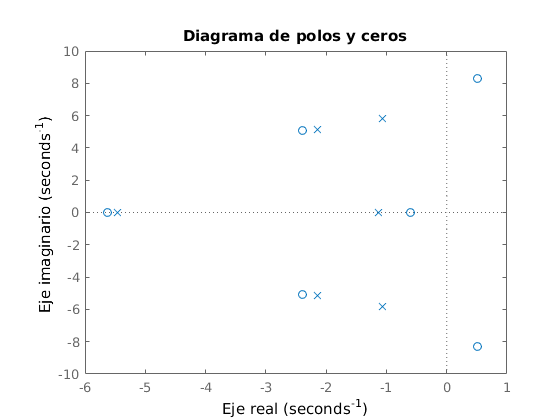
\includegraphics[width=0.6\textwidth]{pictures/Ejercicio5/diag_polos_ceros}
	\caption{Gráfica del mapa de polos y ceros del sistema G}
	\label{fig:diag_polos_ceros}
\end{figure} 



En el siguiente segmento de código se muestra la obtención de la respuesta del sistema propuesto al
estado x indicado. En la gráfica de la figura \ref{fig:respuesta_estado_x}, se muestra esta respuesta
del sistema.
\begin{lstlisting}[style=Matlab-editor, basicstyle=\mlttfamily]
  % Respuesta natural al estado x
  x = [-1; -0.5; 2; -1; 1; 3];
  [Y1,T] = initial(G,x);
  figure
  plot(T,Y1)
\end{lstlisting}

Es importante destacar que el comando \texttt{initial} genera la función correspondiente a la
respuesta del sistema ante un estado inicial, pero tomando la entrada de dicho sistema como nula. 

\begin{figure}[ht!]
	\centering
	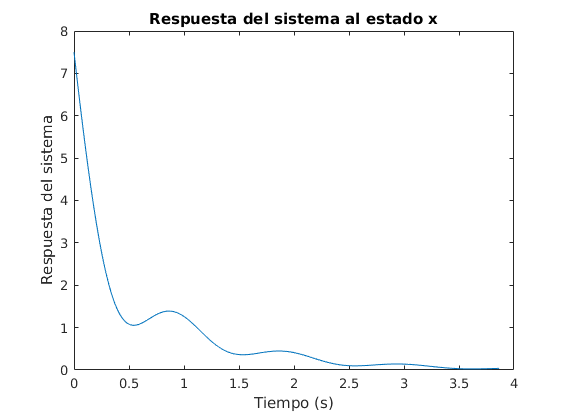
\includegraphics[width=0.6\textwidth]{pictures/Ejercicio5/respuesta_estado_x}
	\caption{Gráfica de la respuesta del sistema G al estado x}
	\label{fig:respuesta_estado_x}
\end{figure} 




A continuación  se muestra la sección del script de MATLAB correspondiente a la obtención de la 
respuesta del sistema ante una entrada impulso. En la gráfica de la figura \ref{fig:respuesta_impulso} 
se muestra dicha respuesta del sistema.

\begin{lstlisting}[style=Matlab-editor, basicstyle=\mlttfamily]
  % Respuesta al impulso 
  [Y2,T] = impulse(G);
  figure
  plot(T,Y2)
\end{lstlisting}

En este caso, la función \texttt{impulse} genera la respuesta del sistema ante esta entrada tomando
como estado inicial al estado cero. 

\begin{figure}[ht!]
	\centering
	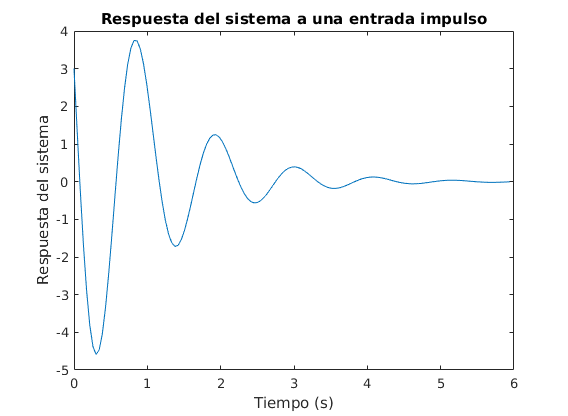
\includegraphics[width=0.6\textwidth]{pictures/Ejercicio5/respuesta_impulso}
	\caption{Gráfica de la respuesta del sistema G a una entrada impulso}
	\label{fig:respuesta_impulso}
\end{figure} 




En el siguiente segmento de código se presenta la generación de la gráfica que muestra la respuesta
del sistema ante una entrada escalón. En la figura \ref{fig:respuesta_escalon} se puede observar
dicha gráfica.

\begin{lstlisting}[style=Matlab-editor, basicstyle=\mlttfamily]
  % Respuesta a una entrada escalon
  [Y3,T] = step(G);
  figure
  plot(T,Y3)
\end{lstlisting}

En este caso, al igual que con el comando \texttt{impulse}, la función \texttt{step} calcula la respuesta del
sistema tomando como estado inicial al estado cero.

\begin{figure}[ht!]
	\centering
	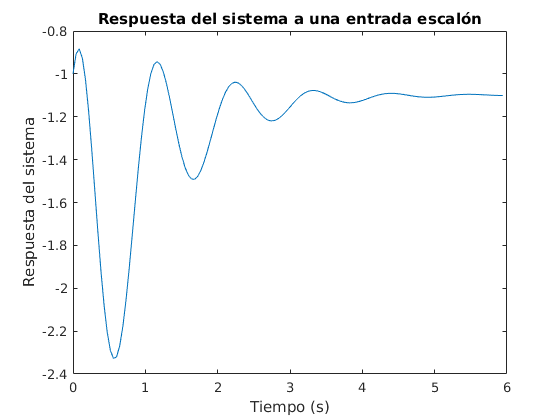
\includegraphics[width=0.6\textwidth]{pictures/Ejercicio5/respuesta_escalon}
	\caption{Gráfica de la respuesta del sistema G a una entrada escalón}
	\label{fig:respuesta_escalon}
\end{figure} 


Para el siguiente punto de la práctica, en donde se solicitaba obtener la gráfica de la respuesta
del sistema ante cierta onda cuadrada, se procedió en primer lugar a generar esta señal cuadrada según
las características indicadas, tales como el período de la misma.

En las siguientes líneas de código se muestra como se obtuvo dicha onda por medio del comando
\texttt{gensig}. En la figura \ref{fig:onda_cuadrada}, se muestra dicha señal.

\begin{lstlisting}[style=Matlab-editor, basicstyle=\mlttfamily]
  % Onda cuadrada
  [sig, T] = gensig('square', 15, 60, 0.01);
  figure
  plot(T, sig)
\end{lstlisting}

\begin{figure}[ht!]
	\centering
	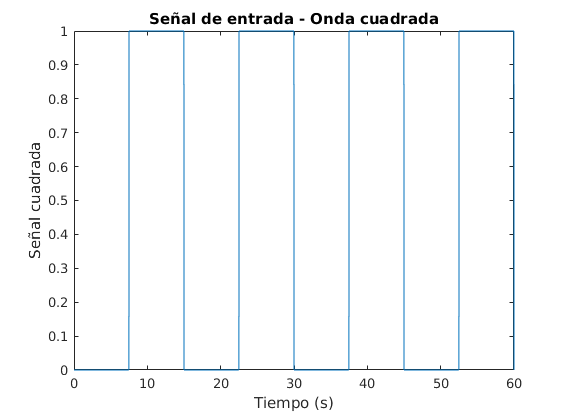
\includegraphics[width=0.6\textwidth]{pictures/Ejercicio5/onda_cuadrada}
	\caption{Señal cuadrada de entrada al sistema G}
	\label{fig:onda_cuadrada}
\end{figure} 


Una vez generada la señal cuadrada, se procedió a obtener la respuesta del sistema ante dicha señal
como entrada, tal como se muestra en la siguiente sección de código.

\begin{lstlisting}[style=Matlab-editor, basicstyle=\mlttfamily]
  % Respuesta a la onda cuadrada
  Y4 = lsim(G, sig, t);
  figure
  plot(T,Y4)
\end{lstlisting}

En la figura \ref{fig:respuesta_onda_cuadrada}, se muestra la gráfica de esta respuesta calculada a
partir de la función \texttt{lsim}, la cual permite simular la respuesta del sistema ante cierta
entrada indicada como parámetro, en este caso \texttt{sig}. 

\begin{figure}[ht!]
	\centering
	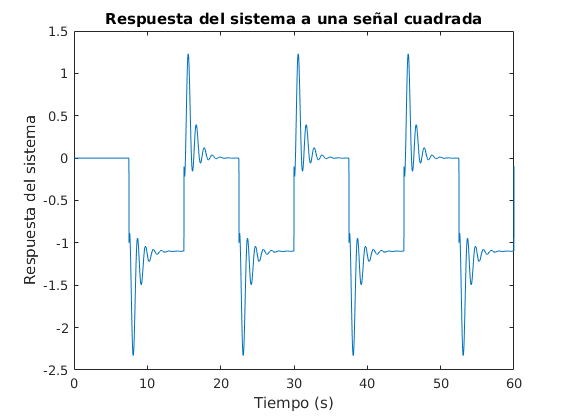
\includegraphics[width=0.6\textwidth]{pictures/Ejercicio5/respuesta_onda_cuadrada}
	\caption{Gráfica de la respuesta del sistema G a la señal cuadrada}
	\label{fig:respuesta_onda_cuadrada}
\end{figure} 

Finalmente, se obtuvo una expresión para la función de transferencia asociada al sistema. Para esto,
en primer lugar se utilizó la función \texttt{ss2tf}, la cual calcula los vectores de los
coeficientes polinomiales tanto del denominador como del numerador de la función de transferencia, 
a partir de cierta representación en el espacio de estados. 

Luego, se empleó la función \texttt{tf} para obtener propiamente la función de transferencia, a partir estos 
vectores de coeficientes del numerador ($G_{num}$) y denominador ($G_{den}$). La función
\texttt{minreal}, toma esta función de transferencia obtenida y realiza todas las simplificaciones
posibles correspondientes a la cancelación de los polos y ceros en la misma.

En el siguiente segmento de código, se muestran los pasos descritos previamente, para el cálculo de
la función de transferencia mostrada en la figura \ref{fig:func_transferencia_H}, que corresponde al resultado obtenido en la
ventana de comandos de MATLAB.

\begin{lstlisting}[style=Matlab-editor, basicstyle=\mlttfamily]
  % Funcion de transferencia
  [Gnum, Gden] = ss2tf(A,B,C,D,1);
  H = minreal(tf(Gnum, Gden))
\end{lstlisting}

\begin{figure}[ht!]
	\centering
	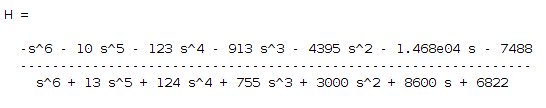
\includegraphics[width=0.6\textwidth]{pictures/Ejercicio5/func_transferencia}
	\caption{Función de transferencia H asociada al sistema representado por G}
	\label{fig:func_transferencia_H}
\end{figure} 


\section{Ejercicio 6}

Se deben encontrar todas las soluciones reales de la función \ref{eq:ecuacion_ejercicio_6}, sin embargo no se puede analizar toda la recta numérica, se debe tomar únicamente una porción. Para esto se calculan los límites de la función en $-\infty$ y $\infty$. 

\begin{equation}
y(x)=x^3+x^2+6x+55cos(x)-10xe^{0.2x}-x^2e^{-0.3x}
\label{eq:ecuacion_ejercicio_6}
\end{equation}

Entonces:
$\lim_{x\to\infty} y(x)=-\infty
\lim_{x\to -\infty} y(x)=-\infty $

Entonces se toma $x$ en el intervalo $[-5000, 5000]$. De la gráfica de la función (ver figura \ref{fig:ejercicio_6_grafica}), se nota que en este intervalo están todas las soluciones.

Para encontrar la solución de la ecuación, se procede a utilizar el método de la falsa posición. Sin embargo este método solamente sirve para encontrar una solución, entonces se hace una ligera adaptación, para poder encontrar todas las soluciones. Se crea un vector x que toma valores desde $-5000$ hasta $5000$ en intervalos de $0.01$. Luego se calcula el vector y asociado, utilizando el criterio en (\ref{eq:ecuacion_ejercicio_6}). Se itera sobre cada entrada de y y se determina si entre esta entrada y la anterior hay un cambio de signo. Si no hay cambio de signo se pasa a la siguiente entrada, pero si sí lo hay, entonces se sabe que entre estos dos puntos existe una solución, entonces se utiliza el método de falsa posición entre estos dos puntos para econtrar las soluciones. 

El método de la falsa posición es recursivo, entonces para esto se define una función recursiva que es llamada en el script principal. En esta función (solucionParticular) se implementa el método de falsa posición descrito en el folleto de análisis. Se reciben los puntos iniciales $(x_l, y_l)$ y $(x_u, y_u)$, si la multiplicación de ambos está lo suficientemente cerca de $0$ (menor a $0.0000001$), entonces se considera que es una solución. Si la multiplicación de ambos no es tan pequeña entonces se calcula el nuevo punto $(x_r, y_r)$, y se calcula solucionParticular entre $x_r$ y $x_l$ si entre ellos hay cambio de signo, o entre $x_r$ y $x_u$ si el cambio está entre estos. 

En el script general, cada vez que se encuentra una solución, se agrega al final de un vector. Cada vez que se agrega una solución el vector crece, esto es porque a priori no se sabe la cantidad de soluciones, entonces se utiliza un vector de tamaño variable. Al final de iterar en cada entrada se obtienen las siguientes soluciones: -1.5206, 1.4455, 4.3645, 17.4701.

\begin{figure}
	\centering
	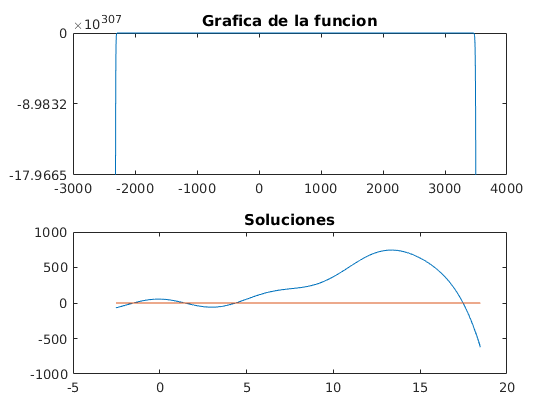
\includegraphics[width=0.5\textwidth]{pictures/ejercicio_6_grafica}
	\caption{Gráfica de la función en (\ref{eq:ecuacion_ejercicio_6})}
	\label{fig:ejercicio_6_grafica}
\end{figure} 

\subsection{Código ejercicio 6}
Script principal:
\lstinputlisting[style=Matlab-editor, basicstyle=\mlttfamily]{Ejercicio6.m}
Función derivadaEstados
\lstinputlisting[style=Matlab-editor, basicstyle=\mlttfamily]{solucionParticular.m}


\end{document}